\subsection{Thuật toán DES}
\subsubsection{Lịch sử hình thành}
\begin{itemize}
    \item Thuật toán mã khối DES (Data Encryption Standard) là một thuật toán mã khối với kích thước khối 64 bít và kích thước khóa 56 bít, được công bố chính thức bởi Tổ chức Tiêu chuẩn xử lý thông tin liên bang Hoa Kỳ (FIPS) vào tháng 11/1976 và được xuất bản trong tài liệu FIPS PUB 46 (01/1977) \cite{Khanh2014}.
    \item Tiền thân của thuật toán DES là thuật toán Lucifer, một thuật toán do IBM phát triển. Cuối năm 1976, DES được chọn làm chuẩn mã hóa dữ liệu của Hoa Kỳ, sau đó được sử dụng rộng rãi trên toàn thế giới trong lĩnh vực an toàn, bảo mật thông tin trên môi trường số \cite{Khanh2014}.
\end{itemize}
\subsubsection{Thuật toán và lưu đồ hoạt động mã hóa dữ liệu DES}
\begin{itemize}
    \item Input: Khối độ dài 64 bits và khóa là 56 bits.
    \item Output: Đầu ra 64 bits.
    \begin{figure}[H]
        \centering
        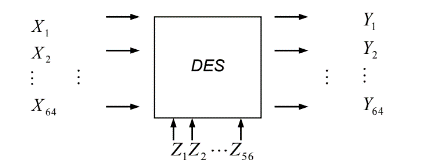
\includegraphics{D:/trang/mật mã/báo cáo/Ảnh/hiền/lưu đồ des.png}
        \caption{Lưu đồ hoạt động DES}
    \end{figure}
\end{itemize}
Thuật toán DES được sử dụng để mã hóa và giải mã các block (khối) dữ liệu 64 bit dựa trên một key (khóa mã) 64 bit.\\
\underline{Chú ý:}  Các block được đánh số thứ tự bít từ trái sang phải và bắt đầu từ 1, bit đầu tiên bên trái là bit số 1 và bit cuối cùng bên phải là bit số 64.\\
\indent Quá trình giải mã và mã hóa sử dụng cùng một key nhưng thứ tự phân phối các giá trị các bit key của quá trình giải mã ngược với quá trình mã hóa.
DES được cấu tạo bởi 16 bước lặp với bước lặp cơ sở gọi hàm chuyển đổi phi tuyến $f$ (có thể hiểu là việc tính toán dựa trên key); 16 bước lặp này được kẹp vào giữa hai tác tử giao hóa IP và IP$^{-1}$. Một block dữ liệu sẽ được hóan vị khởi tạo (Initial Permutation) IP trước khi thực hiện tính toán mã hóa với key, cuối cùng kết quả tính toán với key sẽ được hóa vị lần nữa - đây là hoán vị đảo của hoán vị khởi tạo được gọi là IP$^{-1}$. Hàm cơ sở $f$ là nguồn gốc của sức mạnh bảo mật trong thuật toán DES. Sự lặp lại nhiều lần các bước lặp với tác dụng của f là nhằm tăng cường \textbf{tính nhập nhằng và khuếch tán} (Confusion \& Diffusion) đã có trong $f$.
Hàm $KS$, gọi là hàm phân phối key (Key Schedule). Đây là hàm tạo ra các khóa vòng (Round Key) cho các lần lặp mã hóa. Có tất cả 16 khóa vòng từ $K_1$ đến $K_{16}$ \cite{Khanh2014}.
\begin{figure}[H]
    \centering
    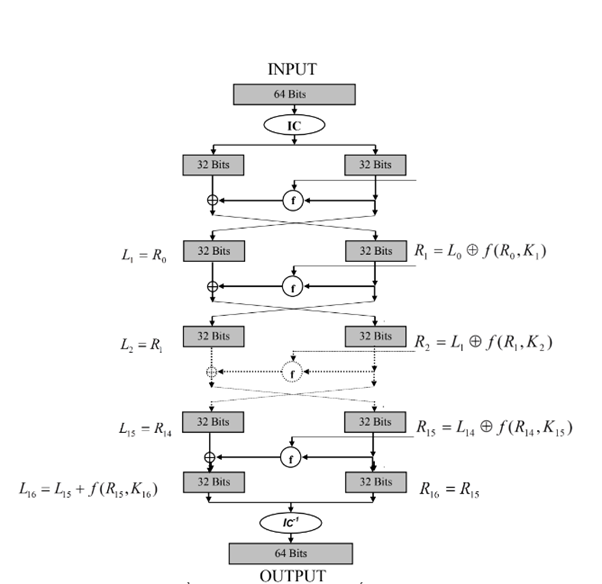
\includegraphics[width=\textwidth,height=15cm]{D:/trang/mật mã/báo cáo/Ảnh/hiền/lưu đồ des-1.png}
    \caption{Sơ đồ sinh mã DES}
\end{figure}
Trên đây là sơ đồ sinh mã DES với cấu trúc 16 vòng lặp.
\subsubsection{Hoán vị khởi tạo - $IP$}
Hoán vị là thay đổi vị trí các bit trong một chuỗi giá trị nhưng không làm thay đổi giá trị của các bit này. Đây là bước đầu tiên trong quy trình mã hóa dữ liệu. 64 bit dữ liệu đầu vào, gọi là Plaintext, sẽ được hoán vị theo bảng mô tả sau đây.
\begin{figure}[H]
    \centering
    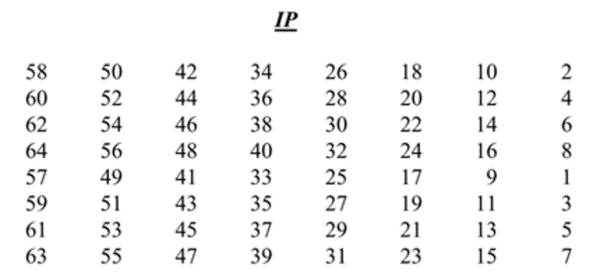
\includegraphics[width=\textwidth]{D:/trang/mật mã/báo cáo/Ảnh/hiền/IP.png}
    \caption{Bảng tra cứu $IP$}
\end{figure}
\indent Chuỗi bit đầu vào được đánh số từ 1 đến 64 (tính từ trái qua phải). Sau đó, các bit này được thay đổi vị trí như sơ đồ $IP$, bit số 58 được đặt vào vị trí đầu tiên, bit số 50 được đặt vào vị trí thứ 2. Cứ như vậy, bit thứ 7 được đặt vào vị trí cuối cùng.\\
\indent Sau hoán vị, chuỗi bit mới được phân ra làm hai đoạn, mỗi đoạn 32 bit để bắt đầu vào quy trình tính toán mã hóa với key. 
\begin{itemize}
    \item Đoạn bên trái kí hiệu là $L$: gồm các bit từ bit số 1 đến bit số 32.
    \item Đoạn bên phải kí hiệu là $R$: các bit từ bit số 33 đến bit số 64.
    \item Đoạn $L$ của lần tính toán sau sẽ chính là đoạn $R$ của lần tính toán trước. 
    \item Đoạn $R$ của lần tính toán sau được tính như sau:
    \[\begin{gathered}
  {L_{n + 1}} = {R_n} \hfill \\
  {R_{n + 1}} = {L_n} \oplus f({R_n},{K_{n + 1}}) \hfill \\ 
\end{gathered} \]
\end{itemize}
 \subsubsection{Hàm mã khóa $f(R,K)$}
\begin{figure}[H]
	\centering
	\includegraphics[scale=0.6]{"Ảnh/hiền/biến đổi E"}
	\caption{Sơ đồ biến đổi cụ thể hàm $f$}
	\label{fig:bien-oi-e}
\end{figure}
Đây là sơ đồ biến đổi cụ thể của hàm $f$. Trước hết, 32 bit của thành phần $R_{i-1}$ được mở rộng thành 48 bit thông qua biến đổi $E$ (Expansion: mở rộng với sự lại 1 số bit). Dưới đây là bảng tra cứu $E$: 
\begin{figure}[H]
	\centering
	\includegraphics[scale=0.6]{"Ảnh/hiền/tra cứu E"}
	\caption{Bảng tra cứu $E$}
	\label{fig:tra-cuu-e}
\end{figure}
Sau khi thực hiện tra cứu $E$, giá trị 48 bit được XOR với 48 bit khóa $K_i$. Tiếp theo, 48 bit kết quả sẽ được phân thành 8 nhóm 6 bit. Mỗi nhóm này sẽ đi vào một biến đổi đặc biệt gọi là biến đổi S-box (có 8 S-box khác nhau ứng với mỗi nhóm 6 bit). \\
\indent Mỗi S-box bao gồm 4 bảng biến đổi dòng, thực chất là một biến đổi hoán vị cho 16 tổ hợp của 4 bits. Trong 6 bit đầu vào thì 2 bit ngoài cùng (bit 1 và bit 6) được dùng để chỉ định 1 trong 4 bảng biến đổi dòng này, vì thế chúng được gọi là các bit điều khiển trái và phải (CL và CR). Còn lại 4 bit chính (từ bit 2 đến bit 5) của nhóm 6 bit đầu vào sẽ là tổ hợp 4 bit bị biến đổi. \\
Ví dụ: Bảng biến đổi $S_{5}$ với 6 bit đầu vào là 011011:
\begin{figure}[H]
    \centering
    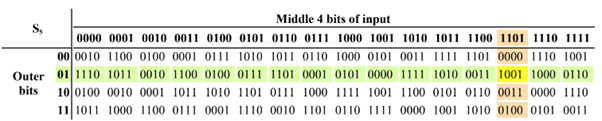
\includegraphics[width=\textwidth]{D:/trang/mật mã/báo cáo/Ảnh/hiền/s5.png}
    \caption{Ví dụ tra cứu $S_5$}
\end{figure}
Qua bước chuyển đổi với các hàm S-box, kết quả thu được là một giá trị 32 bit. Giá trị này sẽ được hoán vị lại theo hàm hoán vị $P$ để đưa ra kết quả cuối cùng của hàm $f$.
\begin{figure}[H]
	\includegraphics[scale=0.6]{"Ảnh/hiền/hoán vị P"}
	\caption{Bảng tra cứu hàm hoán vị $P$}
	\label{fig:hoan-vi-p}
\end{figure}
Giá trị 32 bit thu được từ các chuyển đổi với hàm lựa chọn S sẽ được đánh số từ 1 đến 32 theo thứ tự từ trái qua phải. Theo bảng hoán vị $P$, bit đầu tiên sau hoán vị sẽ là bit số 16, bit thứ 2 sẽ là bit số 7 và bit cuối cùng sẽ là bit số 25.Hàm tính toán mã hóa $f(R, K)$ được định nghĩa như sau:
\[\begin{gathered}
  f(R,K) = P({S_1}({B_1}){S_2}({B_2})...{S_8}({B_8})) \hfill \\
  {B_1}{B_2}...{B_8} = K \oplus E(R) \hfill \\ 
\end{gathered} \]
Trong đó: 
\begin{itemize}
    \item $P()$ là phép hoán vị $P$.
    \item $S_{n}$ là phép chuyển đổi block $n$ ($n$ chạy từ 1 đến 8 với hàm lựa chọn $S$).
    \item $B_{n}$ là block 6 bit thứ $n$ ($n$ chạy từ 1 đến 8). Block này lấy từ phép toán XOR giữa khóa vòng $K$ và giá trị hàm $E(R)$.
\end{itemize}
\subsubsection{Hàm phân phối Key (Key Schedule)}
Một key có 64 bit nhưng chỉ có 56 bit được sử dụng để thực hiện tính toán giá trị khóa vòng. Key được chia làm 8 byte. Các bit ở vị trí 8, 16, 32, 40, 48, 56 và 64 là các bit parity được sử dụng để kiểm tra độ chính xác của key theo từng byte vì khi key được phân phối trên đường truyền đến bộ mã hóa giải mã thì có thể xảy ra lỗi. Parity được sử dụng là parity lẻ (odd parity). Thuật toán tính khóa vòng được mô tả bởi hình dưới đây:
\begin{figure}[H]
	\centering
	\includegraphics[scale=0.7]{"Ảnh/hiền/khóa k"}
	\caption{Thuật toán tính khóa vòng}
	\label{fig:khoa-k}
\end{figure}
Key gốc sẽ được thực hiện hoán vị lựa chọn PC-1. Key được đánh số từ 1 đến 64 theo thứ tự từ trái qua phải.
\begin{figure}[H]
    \centering
    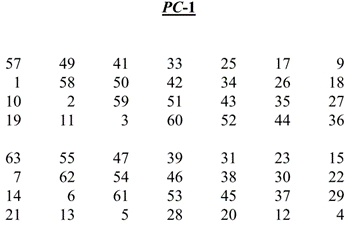
\includegraphics{Ảnh/hiền/pc-1.png}
    \caption{Bảng tra cứu PC-1}
\end{figure}
Bảng hoán vị lựa chọn PC-1 có hai phần. Phần đầu dùng để xác định giá trị $C_0$ và phần sau dùng để xác định giá trị $D_0$. Theo bảng trên thì $C_0$ là chuỗi bit có thứ tự là 57, 49, 41, ..., 36 lấy từ key gốc, $D_0$ là chuỗi bit có thứ tự là 63, 55, 47, ..., 4 lấy từ key gốc.\cite{Khanh2014}\\
\indent Sau khi xác định được giá trị ban đầu để tính key là $C_0$ và $D_0$ thì các khóa vòng $K_n$ (với $n$ từ 1 đến 16) sẽ được tính theo nguyên tắc giá trị của khóa vòng thứ $n$ sẽ được tính từ giá trị khóa vòng thứ $n-1$.
\[{K_n} = P{C_{ - 2}}({C_n}{D_n})\]
Trong đó: $C_{n}$ và $D_{n}$ được tạo từ $C_{n-1}$ và $D_{n-1}$ bằng cách dịch trái các giá trị này với số bit được quy định \cite{Khanh2014}.
\begin{figure}[H]
	\centering
	\includegraphics[scale=1]{"Ảnh/hiền/dịch trái"}
	\caption{Bảng quy định số bit dịch trái khi tính khóa vòng}
	\label{fig:dich-trai}
\end{figure}
Ví dụ, theo bảng trên, $C_{3}$ và $D_{3}$ có được từ $C_{2}$ và $D_{2}$ bằng cách dịch trái 2 bit. Hay $C_{16}$ và $D_{16}$ có được từ $C_{15}$ và $D_{15}$ bằng cách dịch trái 1 bit.
\begin{figure}[H]
	\centering
	\includegraphics[width=\textwidth]{"Ảnh/hiền/quy tắc dịch trái"}
	\caption{Minh họa phép dịch trái khi tính khóa vòng}
	\label{fig:quy-tac-dich-trai}
\end{figure}
Sau khi tính được $C_n$ và $D_n$ thì chuỗi $C_nD_n$ sẽ được đánh số từ 1 đến 56 theo thứ tự từ trái sang phải và được hoán vị lựa chọn lần 2 theo bảng hoán vị PC-2.
\begin{figure}[H]
    \centering
    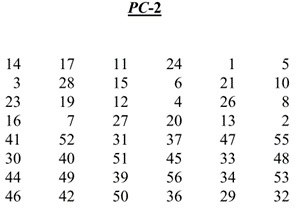
\includegraphics{D:/trang/mật mã/báo cáo/Ảnh/hiền/pc-2.png}
    \caption{Bảng tra cứu PC-2}
\end{figure}
Như vậy bit đầu tiên của khóa vòng $K_n$ là bit số 14 của chuỗi $C_nD_n$, bit thứ 2 là bit số 17 của chuỗi $C_nD_n$ và bit cuối cùng là bit số 32 của chuỗi $C_nD_n$.

\subsubsection{Hoán vị khởi tạo $IP^{-1}$}
Đây là bước cuối cùng để tạo ra giá trị mã hóa. Giá trị của lần lặp mã hóa cuối cùng sẽ được hoán vị khởi tạo đảo $IP^{-1}$ và tạo ra giá trị mã hóa plaintext.
\begin{figure}[H]
    \centering
    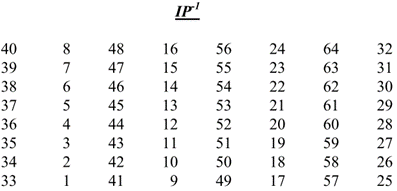
\includegraphics{D:/trang/mật mã/báo cáo/Ảnh/hiền/ip-1.png}
    \caption{Bảng tra cứu hoán vị đảo $IP^{-1}$}
\end{figure}
\subsubsection{Ví dụ về mã hóa DES}
Giả sử ta có dữ liệu cần mã hóa và key là: \\
M = 00123456789abcde (Hex) = 0000 0000 0001 0010 0011 0100 0101 0110 0111 1000 1001 1010 1011 1100 1101 1111. \\
K = 0133457799bbcdff (Hex) = 0000 0001 0011 0011 0100 0101 0111 0111 1001 10001 1011 1011 1100 1100 1111 1111.\\
Từ hai đầu vào này, giá trị của từng bước tính toán mã hóa DES sẽ được minh họa chi tiết sau đây.\cite{Khanh2014}
\begin{enumerate}
    \item Hoán vị khởi tạo - $IP$\\
    Thông điệp M được đánh số vị trí bit từ trái qua phải như sau:
    \begin{figure}[H]
        \centering
        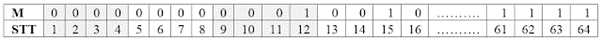
\includegraphics{D:/trang/mật mã/báo cáo/Ảnh/hiền/vs hoán vị.png}
        \caption{Hình ảnh minh họa thông điệp M}
    \end{figure}
    Sắp xếp lại thứ tự các bit của M theo bảng hoán vị $IP$, kết quả có được sau bước này là:
    $IP(M)$ = 98fecc00e054f0aa (Hex) = 1001 1000 1111 1110 1100 1100 0000 0000 1110 0000 0101 0100 1111 0000 1010 1010.
    \item Tính toán giá trị các khóa vòng – KS\\
    Để tính toán hàm mã hóa $f$, chúng ta cần có giá trị khóa cho từng lần lặp mã hóa. Key ban đầu được đánh số thứ tự bit từ trái qua phải.\\
    Sau khi sắp xếp các bit theo bảng hoán vị PC-1 ở trên, kết quả thu được là hai giá trị đầu như sau: 
    \begin{itemize}
        \item $C_{0}$ = f0ccaab (Hex) = 1111 0000 1100 1100 1010 1010 1011. 
        \item $D_{0}$ = aaccf0a (Hex) = 1010 1010 1100 1100 1111 0000 1010. 
    \end{itemize}
    Để tính khóa vòng đầu tiên $K_1$ thì $C_0$ và $D_0$ sẽ được dịch (quay) trái 1 bit. Giá trị thu được sau khi dịch trái là: 
    \begin{itemize}
        \item $C_{1}$ = e199557 (Hex) = 1110 0001 1001 1001 0101 0101 0111 
        \item $D_{1}$ = 5599e15 (Hex) = 0101 0101 1001 1001 1110 0001 0101 
    \end{itemize}
    Hai chuỗi $C_{1}$ và $D_{1}$ được ghép lài thành một chuỗi 56 bit là e1995575599e15. Chuỗi này được hoán vị bằng bảng PC-2 để được giá trị khóa vòng 48 bit thứ nhất $K_1$. 
    \begin{itemize}
        \item $K_1$ = 1b02efdb49a5 (Hex) 
    \end{itemize}
    Để tính khóa vòng $K_2$ thì lấy $C_{1}$ và $D_{1}$ dịch trái với số lượng bit theo bảng ở phần trên, rồi lấy kết quả hoán vị theo bảng PC-2. Quá trình cứ tiếp tục cho đến khóa vòng cuối cùng là $K_{16}$. Kết quả các khóa vòng 48 bit thu được là:
    \begin{itemize}
        \item $K_2$ = 69aed925ae66 (Hex) 
        \item $K_3$ = 55fc8ab4acd2 
        \item $K_4$ = 72add2ad8657 
        \item $K_5$ = 7cec071fe6c2 
        \item $K_6$ = 63a51e3cc545 
        \item $K_7$ = 6c84b78ae4c6 
        \item $K_8$ = f7883aece781 
        \item $K_9$ = c0dbeb27b839 
        \item $K_{10}$ = b1f347631d76 
        \item $K_{11}$ = 215fc30d89be 
        \item $_{K12}$ = 7171f5455cd5 
        \item $K_{13}$ = 95c5d14b80fd 
        \item $K_{14}$ = 5743b783đ8d 
        \item $K_{15}$ = bf91850a17b5 
        \item $K_{16}$ = cb3d0bbc7072
    \end{itemize}
    \item Tính hàm mã hóa $f(R,K)$
    Sau bước hoán vị khởi tạo $IP$, giá trị $IP(M)$ sẽ được tách làm hai phần là: 
    \begin{itemize}
        \item $R_{0}$ = e054f0aa (Hex) = 1110 0000 0101 0100 1111 0000 1010 1010. 
        \item $L_{0}$ = 98fecc00 (Hex) = 1001 1000 1111 1110 1100 1100 0000 0000. 
    \end{itemize}
    Giá trị 32 bit của $R_{0}$ được tra qua bảng E để tạo ra một giá trị 48 bit. 
    \begin{itemize}
        \item E($R_{0}$) = 7002a97a1555 (Hex). 
    \end{itemize}
    Giá trị này được XOR với khóa vòng thứ nhất K1 và được kết quả
    \begin{itemize}
        \item XOR(E($R_{0}$), $K_1$) = 6b0046a15cf0 (Hex).
    \end{itemize}
    Giá trị trên được chia thành 8 nhóm theo thứ tự từ trái qua phải, mỗi nhóm 6 bit để đưa đến các bảng $S$.
    \begin{figure}[H]
        \centering
        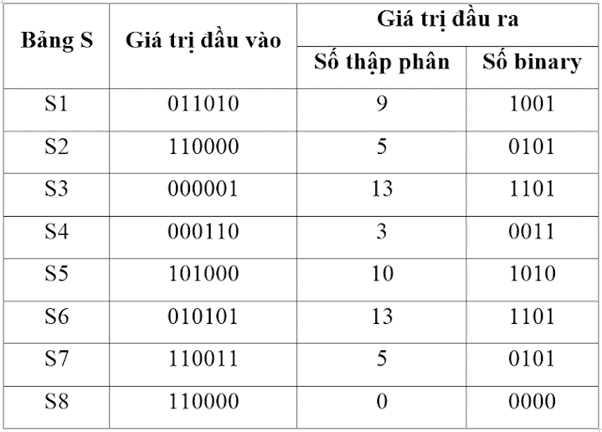
\includegraphics{D:/trang/mật mã/báo cáo/Ảnh/hiền/vd s-box.png}
        \caption{Bảng giá trị của biến đổi S-box}
    \end{figure}
    Các giá trị đầu ra sau bước tra các bảng $S$ sẽ được ghép lại theo thứ tự từ $S_1$ đến $S_8$ để được 1 giá trị 32 bit. 
    \begin{itemize}
        \item $S_1()S_2()S_3()S_4()S_5()S_6()S_7()S_8() = 10010101110100111010110101010000 = 95d3ad50$ (Hex). 
    \end{itemize}
    Giá trị này được hoán vị bằng bảng $P$ để cho ra giá trị của hàm $f$. 
    \begin{itemize}
        \item $f(R_{0},K_1)$ = 97d1619a (Hex) = 1001 0111 1101 0001 0110 0001 1001 1010. 
    \end{itemize}
    Tương tự, ta có giá trị hàm $f$ tại các vòng lặp mã hóa còn lại như sau: 
    \begin{itemize}
        \item $f(R_{1},K_2)$ = 88488d0b (Hex)
        \item $f(R_{2},K_3)$ = da3b2692 
        \item $f(R_{3},K_4)$ = f44950b2 
        \item $f(R_{4},K_5)$ = d83237fd 
        \item $f(R_{5},K_6)$ = afc43b25 
        \item $f(R_6,K_7)$ = 4e5123a2 
        \item $f(R_7,K_8)$ = 6cfdecb8 
        \item $f(R_8,K_9)$ = fb0600b1 
        \item $f(R_9,K_{10})$ = d51508e4 
        \item $f(R_{10},K_{11})$ = fcf67146 
        \item $f(R_{11},K_{12})$ = 704fa3a5 
        \item $f(R_{12},K_{13})$ = 7bfe2806 
        \item $f(R_{13},K_{14})$ = 65fc7a48 
        \item $f(R_{14},K_{15})$ = 513f1d11 
        \item $f(R_{15},K_{16})$ = cbf5252d
    \end{itemize}
    \item Giá trị tại mỗi vòng lặp mã hóa\\
    Giá trị của hàm $f(R,K)$ được sử dụng để tính giá trị $R_n$ và $L_n$ tại mỗi vòng lặp mã hóa theo công thức:
     \[\begin{gathered}
  {L_{n + 1}} = {R_n} \hfill \\
  {R_{n + 1}} = {L_n} \oplus f({R_n},{K_{n + 1}}) \hfill \\ 
\end{gathered} \]
    Thay vào công thức ở trên ta có các kết quả như sau:
    \begin{figure}[H]
        \centering
        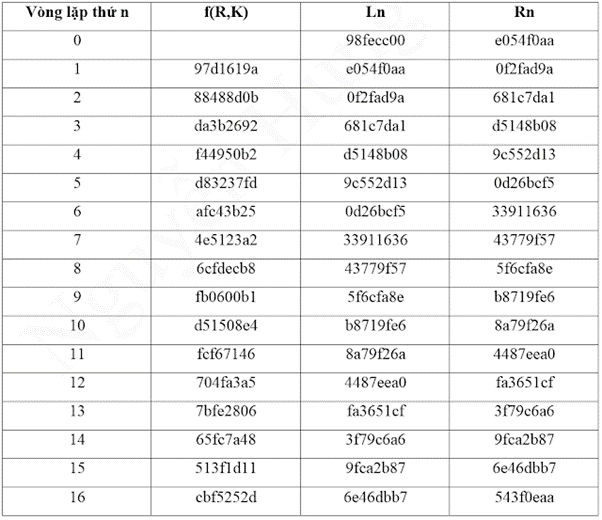
\includegraphics{D:/trang/mật mã/báo cáo/Ảnh/hiền/vs hàm f.png}
        \caption{Mô tả tính toán giá trị tại mỗi vòng lặp mã hóa}
    \end{figure}
    \item Hoán vị khởi tạp đảo $IP^-1$\\
    Giá trị $R_{16}$ và $L_{16}$ của vòng lặp mã hóa cuối cùng sẽ được ghép lại thành một chuỗi 64 bit để thực hiện hoán vị theo bảng $IP^{-1}$.\\
    Kết quả của phép hoán vị này chính là giá trị mã hóa (ciphertext) cần tính.\\
    $IP^{-1}(R_{16}, L_{16})$ = 1abff69d5a93e80b (Hex)\\
    = 0001 1010 1011 1111 1111 0110 1001 1101 0101 1010 1001 0011 1110 1000 0000 1011.

\end{enumerate}
\subsubsection{Thuật toán Giải mã Dữ liệu DES}
Các bước của quá trình giải mã dữ liệu được thực hiện tương tự như quá trình mã hóa dữ liệu. Trong quá trình giải mã có một số thay đổi như sau: 
Đầu vào lúc này là dữ liệu cần giải mã (Ciphertext) và đầu ra là kết quả giải mã được (Plaintext).\\
\indent Khóa vòng sử dụng trong các vòng lặp giải mã có thứ tự ngược với quá trình mã hóa. Nghĩa là, tại vòng lặp giải mã đầu tiên, khóa vòng được sử dụng là $K_{16}$. Tại vòng lặp giải mã thứ 2, khóa vòng được sử dụng là $K_{15}$, và tại vòng lặp giải mã cuối cùng thì khóa vòng được sử dụng là $K_1$ \cite{quan2020}.
\subsubsection{Nhận xét}
\begin{enumerate}
    \item Các thuộc tính của S-box:
    \begin{itemize}
    \item Các bit ra (output bit) luôn phụ thuộc không tuyến tính vào các bit vào (input bit) \cite{Khanh2014}.
    \item Sửa đổi ở một bit vào làm thay đổi ít nhất là hai bit ra \cite{Khanh2014}.
    \item Khi một bit vào được giữ cố định và 5 bit con lại cho thay đổi thì S-boxes thể hiện một tính chất được gọi là \textbf{“Phân bố Đồng nhất” (Uniform Distribution)}: so sánh số lượng bit số 0 và 1 ở các đầu ra luôn ở mức cân bằng. Tính chất này khiến cho việc áp dụng phân tích theo lý thuyết thông kê để tìm cách phá S-boxes là vô ích \cite{Khanh2014}.
    \end{itemize}
    => 3 tính chất này đảm bảo tốt tính chất \textbf{Nhập nhằng và Khuếch tán (Confusion \& Fiffusion)}.\\
    Thực tế, sau 8 vòng lặp tất cả các bit ra của DES sẽ chịu ảnh hưởng của tất cả các bit vào và tất cả các bit của khóa. Hơn nữa sự phụ thuộc này là rất phức tạp. Tuy nhiên sau này một số tấn công mới đã được đề xuất và cho thấy 8 vòng lặp này là chưa đủ để bảo mật \cite{Khanh2014}.
    \item Nhược điểm của thuật toán DES
    \begin{itemize}
    \item Điểm yếu chính trong DES là kích thước khóa, để thực hiện tấn công Brute Force, cần phải kiểm tra  $2^{56}$ khóa khả thi. Do đó, chúng ta nhận thấy:
    \begin{itemize}
        \item Với công nghệ hiện đại, có thể kiểm tra một triệu khóa mỗi giây, nghĩa là cần hơn hai nghìn năm để thực hiện Brute Force bằng máy tính với một bộ xử lý.
        \item Nếu có thể tạo ra máy tính với một triệu chip (xử lý song song), thì có thể kiểm tra toàn bộ không gian khóa trong 20 giờ. Vào năm 1998, máy tính đã có thể tìm thấy khóa DES trong 112 giờ.
        \item Mạng máy tính có thể mô phỏng xử lý song song bằng cách chia không gian khóa giữa nhiều máy tính để thực hiện tấn công Brute Force. Có thể giả định rằng mạng với 42.000 thành viên có thể tìm thấy khóa trong 10 ngày.
        \item Tốc độ của các triển khai phần cứng: Mặc dù các triển khai DES trên phần cứng có thể rất nhanh, nhưng điều này không hẳn là một lợi thế về mặt bảo mật. Nếu phần cứng có thể thực hiện một lượng lớn phép mã hóa và giải mã trong thời gian ngắn, thì thời gian cần thiết để thử tất cả các khóa có thể cũng giảm xuống đáng kể.
        \item Hiệu suất chậm trên phần mềm: DES không được thiết kế ban đầu để chạy trên phần mềm, dẫn đến hiệu suất chậm khi thực thi trên các máy tính thông thường. 
    \end{itemize}
\end{itemize}
\end{enumerate}
\subsubsection{ Mặt hạn chế của DES}
\begin{itemize}
    \item Tốc độ của các triển khai phần cứng: Mặc dù các triển khai DES trên phần cứng có thể rất nhanh, nhưng điều này không hẳn là một lợi thế về mặt bảo mật. Nếu phần cứng có thể thực hiện một lượng lớn phép mã hóa và giải mã trong thời gian ngắn, thì thời gian cần thiết để thử tất cả các khóa có thể cũng giảm xuống đáng kể.
    \item Hiệu suất chậm trên phần mềm: DES không được thiết kế ban đầu để chạy trên phần mềm, dẫn đến hiệu suất chậm khi thực thi trên các máy tính thông thường. 
    \item Điểm yếu chính trong DES là kích thước khóa, để thực hiện tấn công brute force, cần phải kiểm tra $2^{56}$ khóa khả thi \cite{Wikipedia}. Do đó, chúng ta nhận thấy:
 \begin{itemize}
     \item Với công nghệ hiện đại, có thể kiểm tra một triệu khóa mỗi giây, nghĩa là cần hơn hai nghìn năm để thực hiện Brute Force bằng máy tính với một bộ xử lý.
    \item Nếu có thể tạo ra máy tính với một triệu chip (xử lý song song), thì có thể kiểm tra toàn bộ không gian khóa trong 20 giờ. Vào năm 1998, máy tính đã có thể tìm thấy khóa DES trong 112 giờ.
   \item Mạng máy tính có thể mô phỏng xử lý song song bằng cách chia không gian khóa giữa nhiều máy tính để thực hiện tấn công Brute Force. Có thể giả định rằng mạng với 42.000 thành viên có thể tìm thấy khóa trong 10 ngày.

\end{itemize}
    
\end{itemize}